\documentclass[11pt]{article}
\usepackage[a4paper,margin=1in]{geometry}
\usepackage{booktabs}
\usepackage{graphicx}
\usepackage{float}
\usepackage{hyperref}
\usepackage{longtable}
\usepackage{array}

\title{Current Auditory EEG Reproduction Audit Note}
\date{2026-06-18}

\begin{document}
\maketitle

\section*{Purpose}
This note was generated to support external review of the current reproduction state. It records the present evaluation setup, the current result tables, and the training-curve figures that are available for audit.

\section*{Why This Document Is Longer Than A Usual Summary}
The current codebase contains more than one evaluation layer:
\begin{itemize}
\item a historical sample-dataset development layer
\item a newer unified \texttt{reference\_splits} layer
\item exact structural ports whose training mode is not identical to the subject-specific baselines
\end{itemize}
Therefore, a short result table is not sufficient. A reviewer needs enough detail to decide whether an unexpected score is caused by:
\begin{itemize}
\item an implementation bug
\item an optimizer or checkpoint-selection issue
\item a data split mismatch
\item a non-comparable training regime
\end{itemize}

\section*{Evaluation Setup}
The current unified reconstruction datasets are:
\begin{itemize}
\item \texttt{hugo\_sample\_tf64}: development dataset
\item \texttt{weissbart\_tf64}: 13-subject reconstruction dataset
\item \texttt{etard\_tf64}: 20-subject reconstruction dataset
\end{itemize}

For the exact structural ports (\texttt{ADT-exact}, \texttt{VLAAI-exact}), the train/validation/test procedure is:
\begin{enumerate}
\item train on the train split
\item evaluate on the validation split every epoch
\item retain the best validation checkpoint
\item stop after a fixed patience without validation improvement
\item evaluate the retained best-validation checkpoint once on the test split
\end{enumerate}

\paragraph{Important comparability boundary.}
The current main table should not yet be interpreted as a perfect apples-to-apples leaderboard because the training modes differ:
\begin{itemize}
\item \texttt{Ridge}, \texttt{CCA}, \texttt{FCNN}, \texttt{CNN}, and \texttt{EEGNet} are currently run as \emph{subject-specific} models
\item \texttt{ADT-exact} and \texttt{VLAAI-exact} are currently run as \emph{pooled multi-subject} models on the training and validation windows, followed by subject-wise test reporting
\end{itemize}

\section*{Implementation Summary}
\subsection*{Implementation files to inspect}
\begin{longtable}{p{2.2cm} p{4.1cm} p{7.0cm}}
\toprule
Role & Path & Purpose \\
\midrule
\endfirsthead
\toprule
Role & Path & Purpose \\
\midrule
\endhead
unified baseline logic & src/repro/reference\_baselines.py & window construction, linear baselines, CCA, DNN train/eval \\
baseline batch runner & scripts/run\_reference\_baselines.py & per-dataset, per-subject batch execution and metric export \\
ADT exact model & src/repro/adt\_exact.py & exact structural port, pooled sequence training, subject-wise test report \\
VLAAI exact model & src/repro/vlaai\_exact.py & exact structural port, pooled sequence training, subject-wise test report \\
exact batch runner & scripts/run\_reference\_exact\_suite.py & standardized launcher for exact reference runs \\
archive summary builder & scripts/archive\_benchmark\_results.py & aggregates method outputs into comparison CSV and publication-style figures \\
\bottomrule
\end{longtable}

\subsection*{Model protocols}
\begin{longtable}{p{1.4cm} p{1.6cm} p{2.2cm} p{1.8cm} p{1.8cm} p{2.0cm} p{2.4cm} p{2.6cm} p{2.0cm} p{2.8cm}}
\toprule
Family & Model & Implementation & Input & Target & Window/Lag & Optimizer & Selection & Train mode & Notes \\
\midrule
\endfirsthead
\toprule
Family & Model & Implementation & Input & Target & Window/Lag & Optimizer & Selection & Train mode & Notes \\
\midrule
\endhead
unified\_baseline & Ridge & lagged linear decoder & time x 64 & scalar envelope sample & lags 0:50 & sklearn Ridge & best validation correlation over alpha grid & subject-specific & train/val/test are per-subject recording splits \\
unified\_baseline & CCA & CCA reconstruction plus match/mismatch & time x 64 & continuous envelope & lags 0:50, PCA + CCA + ridge reconstruction & sklearn CCA + Ridge & best validation reconstruction correlation & subject-specific & main table uses reconstruction correlation rather than canonical correlation \\
unified\_baseline & FCNN & upstream mldecoders-style DNN & 64 x 50 window & scalar envelope sample & window 50, target at last sample & NAdam lr=1e-4 wd=1e-4 & best validation correlation, patience=10 & subject-specific & per-participant histories available \\
unified\_baseline & CNN & upstream mldecoders CNN & 64 x 50 window & scalar envelope sample & window 50, target at last sample & NAdam lr=1e-2 wd=1e-8 & best validation correlation, patience=10 & subject-specific & F1=8, D=8, F2=64, dropout=0.20 \\
unified\_baseline & EEGNet & EEGNet-style regressor & 64 x 50 window & scalar envelope sample & window 50, target at last sample & NAdam lr=1e-3 wd=1e-4 & best validation correlation, patience=10 & subject-specific & temporal\_filters=8, depth\_multiplier=2, separable\_filters=16, dropout=0.25 \\
exact\_port & ADT-exact & sequence-to-sequence structural port & 320 x 64 window & 320 x 1 envelope sequence & window 320, hop 64 & Adam lr=1e-3 + ReduceLROnPlateau & best pooled validation Pearson checkpoint, patience=10 & pooled multi-subject train/val, subject-wise test report & spatio-temporal conv frontend + anti-causal transformer decoder \\
exact\_port & VLAAI-exact & sequence-to-sequence structural port & 320 x 64 window & 320 x 1 envelope sequence & window 320, hop 64 & Adam lr=1e-3 + ReduceLROnPlateau & best pooled validation Pearson checkpoint, patience=10 & pooled multi-subject train/val, subject-wise test report & shared extractor/output-context modules, 4 blocks \\
\bottomrule
\end{longtable}

\subsection*{Run metadata}
\begin{longtable}{p{2.1cm} p{1.7cm} p{3.0cm} p{1.5cm} p{1.7cm} p{1.5cm} p{1.2cm}}
\toprule
Dataset & Model & Run type & Epochs req. & Epochs done & Best epoch & Histories \\
\midrule
\endfirsthead
\toprule
Dataset & Model & Run type & Epochs req. & Epochs done & Best epoch & Histories \\
\midrule
\endhead
weissbart\_tf64 & FCNN & subject\_specific\_baseline & 100.0 & 13.3 & 2.3 & 13 \\
weissbart\_tf64 & CNN & subject\_specific\_baseline & 92.7 & 15.4 & 4.9 & 13 \\
weissbart\_tf64 & EEGNet & subject\_specific\_baseline & 100.0 & 29.2 & 18.2 & 13 \\
etard\_tf64 & FCNN & subject\_specific\_baseline & 100.0 & 13.7 & 2.6 & 20 \\
etard\_tf64 & CNN & subject\_specific\_baseline & 100.0 & 16.4 & 5.5 & 20 \\
etard\_tf64 & EEGNet & subject\_specific\_baseline & 100.0 & 28.6 & 17.6 & 20 \\
hugo\_sample\_tf64 & ADT-exact & pooled\_exact\_port & 100.0 & 22.0 & 11.0 & 1 \\
hugo\_sample\_tf64 & VLAAI-exact & pooled\_exact\_port & 100.0 & 17.0 & 6.0 & 1 \\
weissbart\_tf64 & ADT-exact & pooled\_exact\_port & 100.0 & 25.0 & 14.0 & 1 \\
weissbart\_tf64 & VLAAI-exact & pooled\_exact\_port & 100.0 & 17.0 & 6.0 & 1 \\
etard\_tf64 & ADT-exact & pooled\_exact\_port & 100.0 & 16.0 & 5.0 & 1 \\
etard\_tf64 & VLAAI-exact & pooled\_exact\_port & 100.0 & 16.0 & 5.0 & 1 \\
\bottomrule
\end{longtable}

\subsection*{Additional audit CSV files}
The following files were generated to support review:
\begin{itemize}
\item \texttt{experiments/summary\_figures/reproduction\_audit\_model\_protocols.csv}
\item \texttt{experiments/summary\_figures/reproduction\_audit\_run\_metadata.csv}
\end{itemize}
The first CSV describes the intended implementation and training mode for each model family. The second CSV describes how many epochs were requested, how many epochs were actually completed, and whether the history comes from a subject-specific average or a single pooled run.

\paragraph{Why the metadata table matters.}
The user explicitly raised concern about very short-looking deep-learning runs. In the current pipeline, a small \texttt{best\_epoch} does not mean the run terminated immediately. It means the best validation checkpoint occurred early and was later restored after patience-based early stopping. The run metadata table is therefore necessary for distinguishing:
\begin{itemize}
\item requested training budget
\item actually completed epochs
\item checkpoint-selection epoch
\end{itemize}

\section*{Current Main Table}
The main unified comparison table is stored in:
\begin{itemize}
\item \texttt{experiments/summary\_figures/unified\_reference\_main\_summary.csv}
\end{itemize}

The current unified results table is reproduced below for direct review:

\begin{longtable}{p{2.1cm} p{1.8cm} p{2.5cm} p{2.1cm} p{1.2cm} p{1.2cm} p{0.9cm}}
\toprule
Dataset & Model & Group & Metric & Mean & Std & N \\
\midrule
\endfirsthead
\toprule
Dataset & Model & Group & Metric & Mean & Std & N \\
\midrule
\endhead
weissbart\_tf64 & Ridge & Unified baseline & test\_pearson & 0.1332 & 0.0290 & 13 \\
weissbart\_tf64 & CCA & Unified baseline & test\_recon\_corr & 0.0931 & 0.0246 & 13 \\
weissbart\_tf64 & FCNN & Unified baseline & test\_pearson & 0.0905 & 0.0419 & 13 \\
weissbart\_tf64 & CNN & Unified baseline & test\_pearson & 0.1228 & 0.0373 & 13 \\
weissbart\_tf64 & EEGNet & Unified baseline & test\_pearson & 0.1465 & 0.0327 & 13 \\
etard\_tf64 & Ridge & Unified baseline & test\_pearson & 0.0982 & 0.0408 & 20 \\
etard\_tf64 & CCA & Unified baseline & test\_recon\_corr & 0.0680 & 0.0232 & 20 \\
etard\_tf64 & FCNN & Unified baseline & test\_pearson & 0.0621 & 0.0198 & 20 \\
etard\_tf64 & CNN & Unified baseline & test\_pearson & 0.0956 & 0.0422 & 20 \\
etard\_tf64 & EEGNet & Unified baseline & test\_pearson & 0.1003 & 0.0411 & 20 \\
weissbart\_tf64 & ADT-exact & Exact structural port & pearson\_metric & 0.1147 & 0.0393 & 13 \\
weissbart\_tf64 & VLAAI-exact & Exact structural port & pearson\_metric & 0.1389 & 0.0335 & 13 \\
etard\_tf64 & ADT-exact & Exact structural port & pearson\_metric & 0.0860 & 0.0445 & 20 \\
etard\_tf64 & VLAAI-exact & Exact structural port & pearson\_metric & 0.1128 & 0.0416 & 20 \\
\bottomrule
\end{longtable}

\begin{figure}[H]
\centering
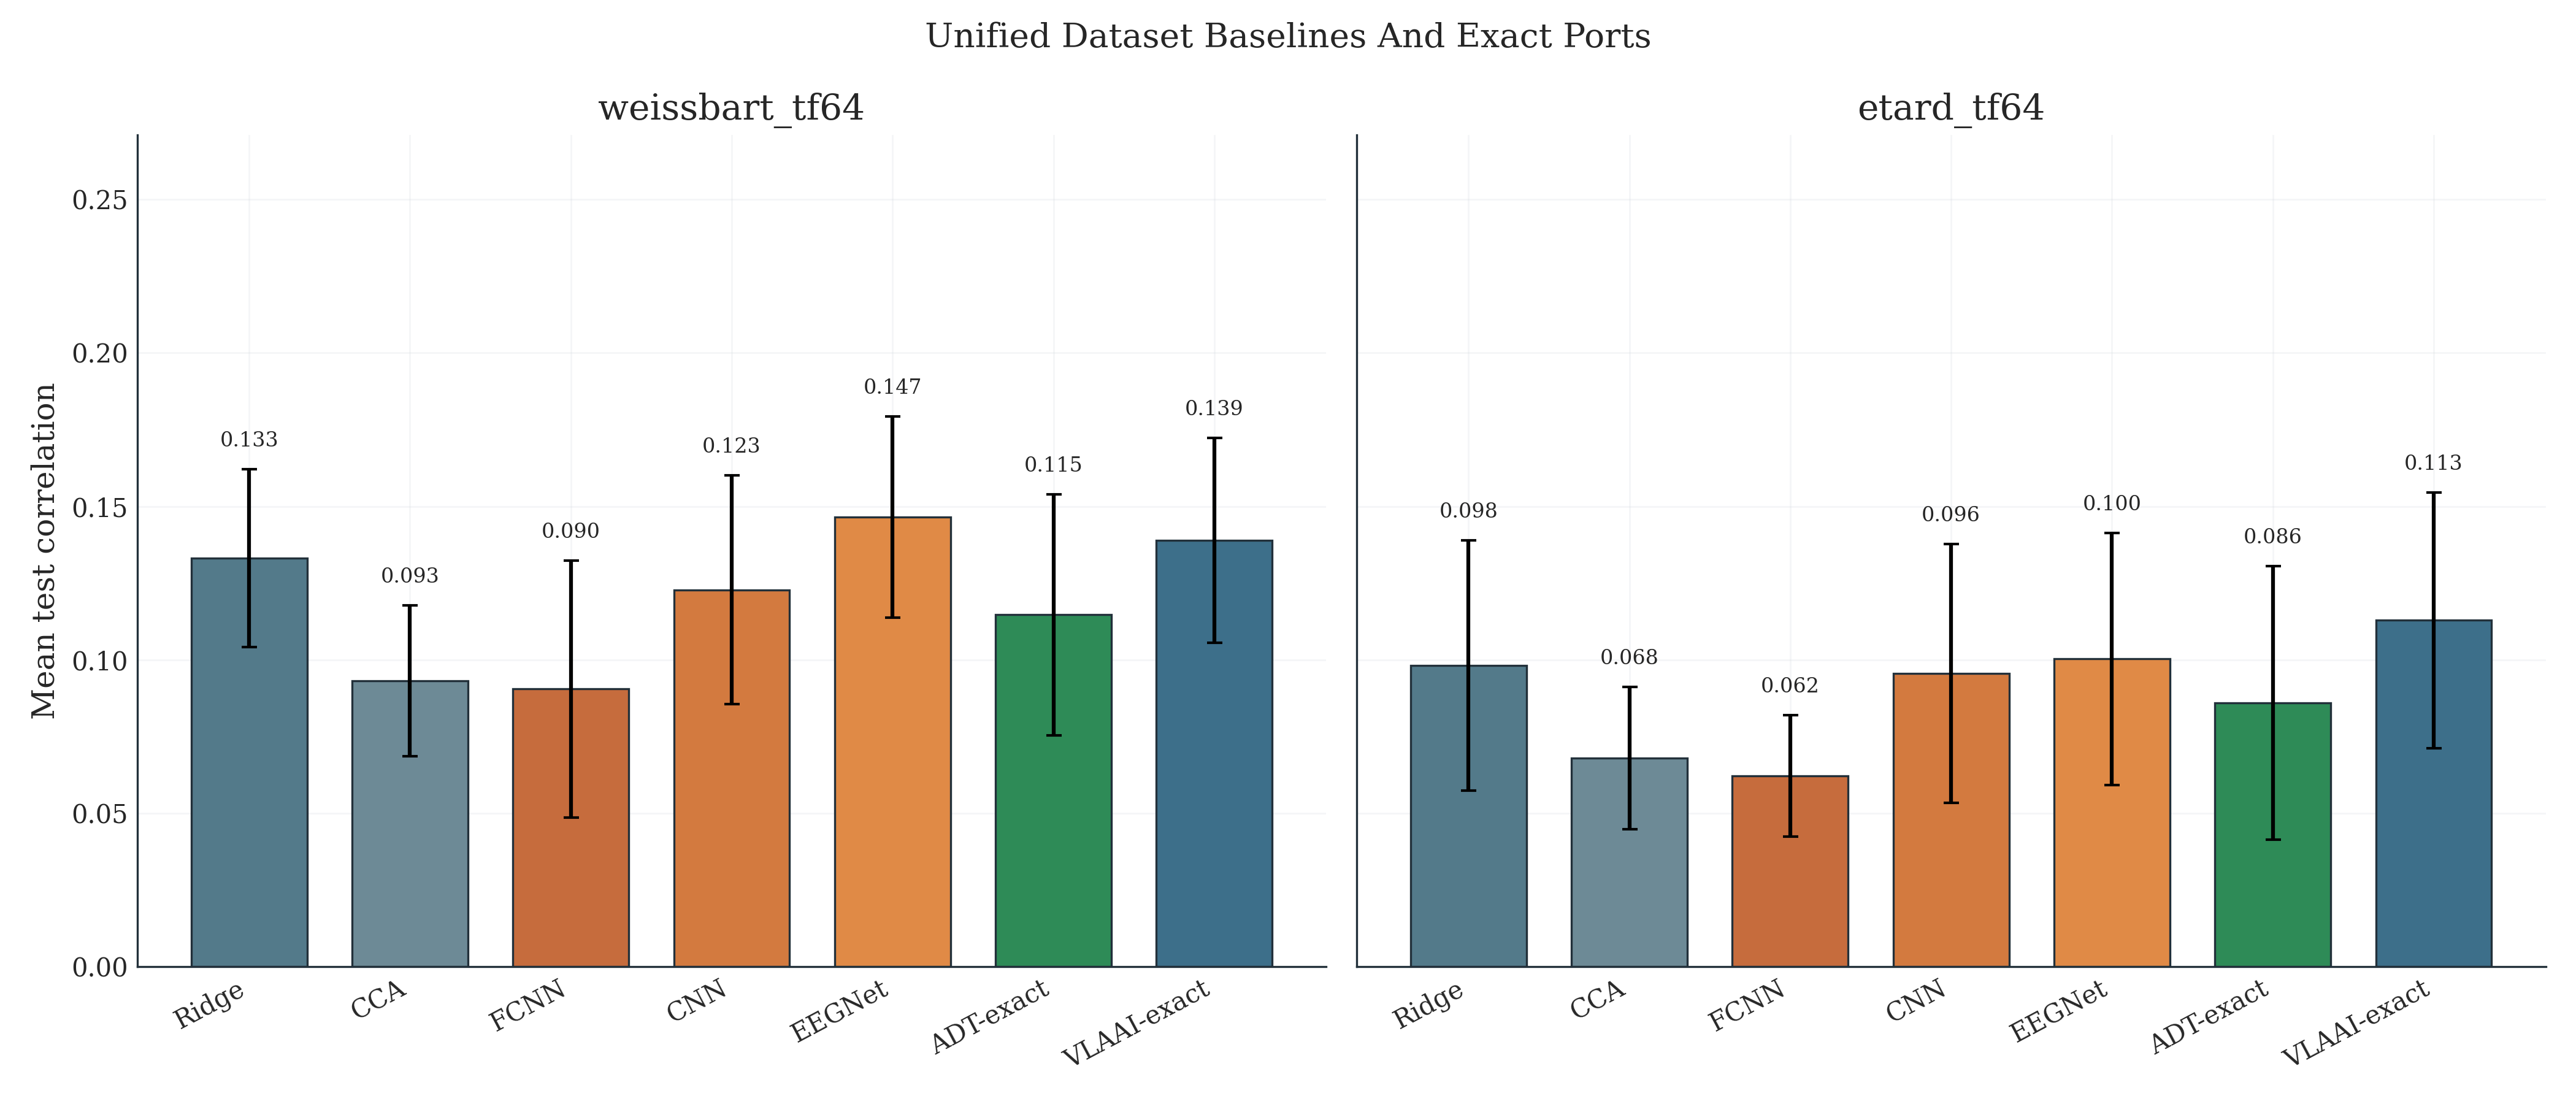
\includegraphics[width=\textwidth]{../experiments/summary_figures/unified_reference_main_overview.png}
\caption{Current unified comparison on Weissbart and Etard.}
\end{figure}

\section*{Training Curves}
The aggregated validation-curve CSV is:
\begin{itemize}
\item \texttt{experiments/summary\_figures/reproduction\_audit\_training\_curves.csv}
\end{itemize}

\begin{figure}[H]
\centering
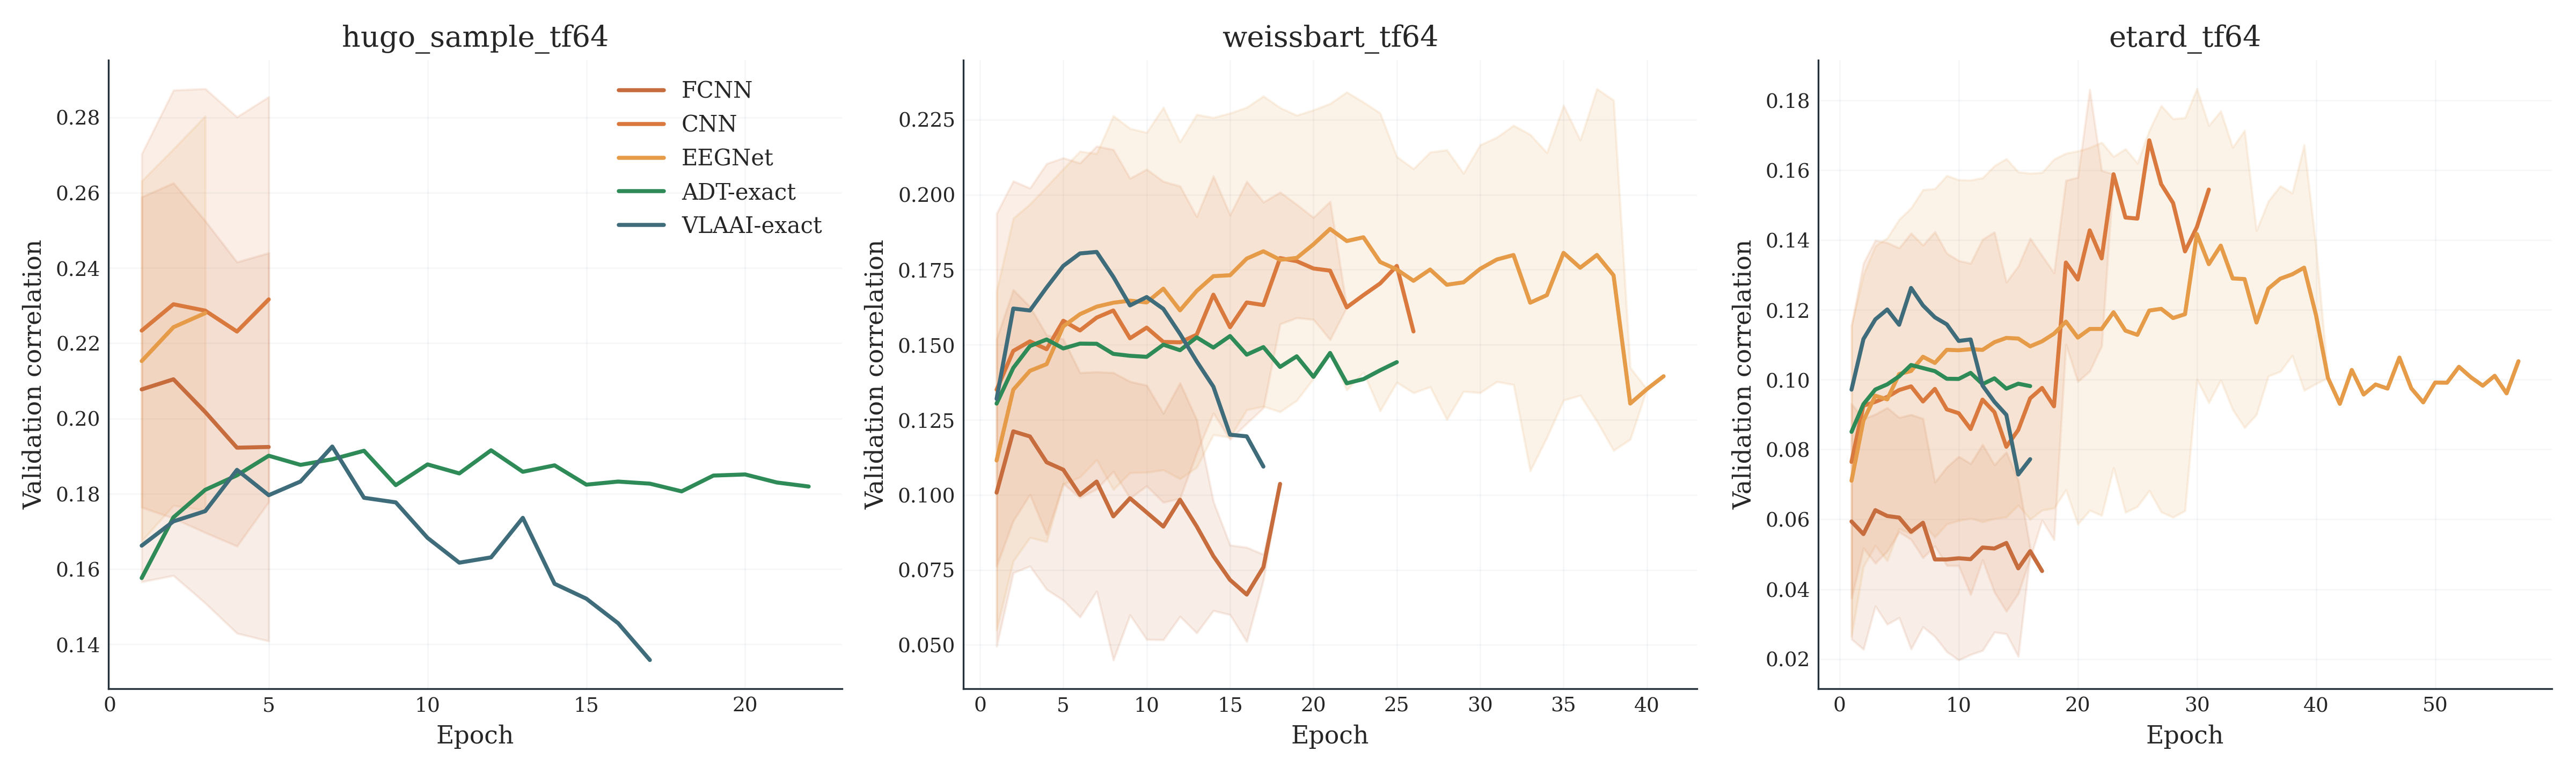
\includegraphics[width=\textwidth]{../experiments/summary_figures/reproduction_audit_training_curves.png}
\caption{Validation curves used for audit. For FCNN/CNN/EEGNet, shaded bands indicate participant-to-participant variation. For exact ports, the curves correspond to the single pooled-data training run.}
\end{figure}

\paragraph{What a reviewer should infer from the curves.}
These curves are useful for identifying at least three different kinds of problems:
\begin{itemize}
\item training instability or collapse
\item apparently healthy optimization with poor final generalization
\item suspiciously flat or very short histories that may indicate a stopping-rule or implementation issue
\end{itemize}
They do not prove correctness by themselves, but they make it much easier to separate implementation failure from protocol mismatch.

\section*{Sample Dataset Method Panorama}
The current sample-only method panorama is stored in:
\begin{itemize}
\item \texttt{experiments/summary\_figures/sample\_all\_methods\_summary.csv}
\end{itemize}

For completeness, the current sample-dataset table is reproduced below:

\begin{longtable}{p{2.1cm} p{2.7cm} p{2.2cm} p{1.2cm} p{1.2cm} p{0.9cm}}
\toprule
Model & Group & Metric & Mean & Std & N \\
\midrule
\endfirsthead
\toprule
Model & Group & Metric & Mean & Std & N \\
\midrule
\endhead
Ridge & Linear / correlation baseline & test\_pearson & 0.1459 &  & 13 \\
AvgDec-Ridge & Linear / correlation baseline & test\_pearson & 0.1220 &  & 13 \\
AvgCorr-Ridge & Linear / correlation baseline & test\_pearson & 0.1449 &  & 13 \\
CCA & Linear / correlation baseline & test\_recon\_corr & 0.1139 &  & 13 \\
FCNN & Neural benchmark & test\_pearson & 0.2058 &  & 13 \\
CNN & Neural benchmark & test\_pearson & 0.2176 &  & 13 \\
EEGNet & Neural benchmark & test\_pearson & 0.2171 &  & 13 \\
VLAAI-lite & Approximate deep port & test\_pearson & 0.1177 &  & 13 \\
ADT-lite & Approximate deep port & test\_pearson & 0.2120 &  & 13 \\
ADT-exact & Exact structural port & pearson\_metric & 0.1447 &  & 13 \\
VLAAI-exact & Exact structural port & pearson\_metric & 0.1477 &  & 13 \\
\bottomrule
\end{longtable}

\begin{figure}[H]
\centering
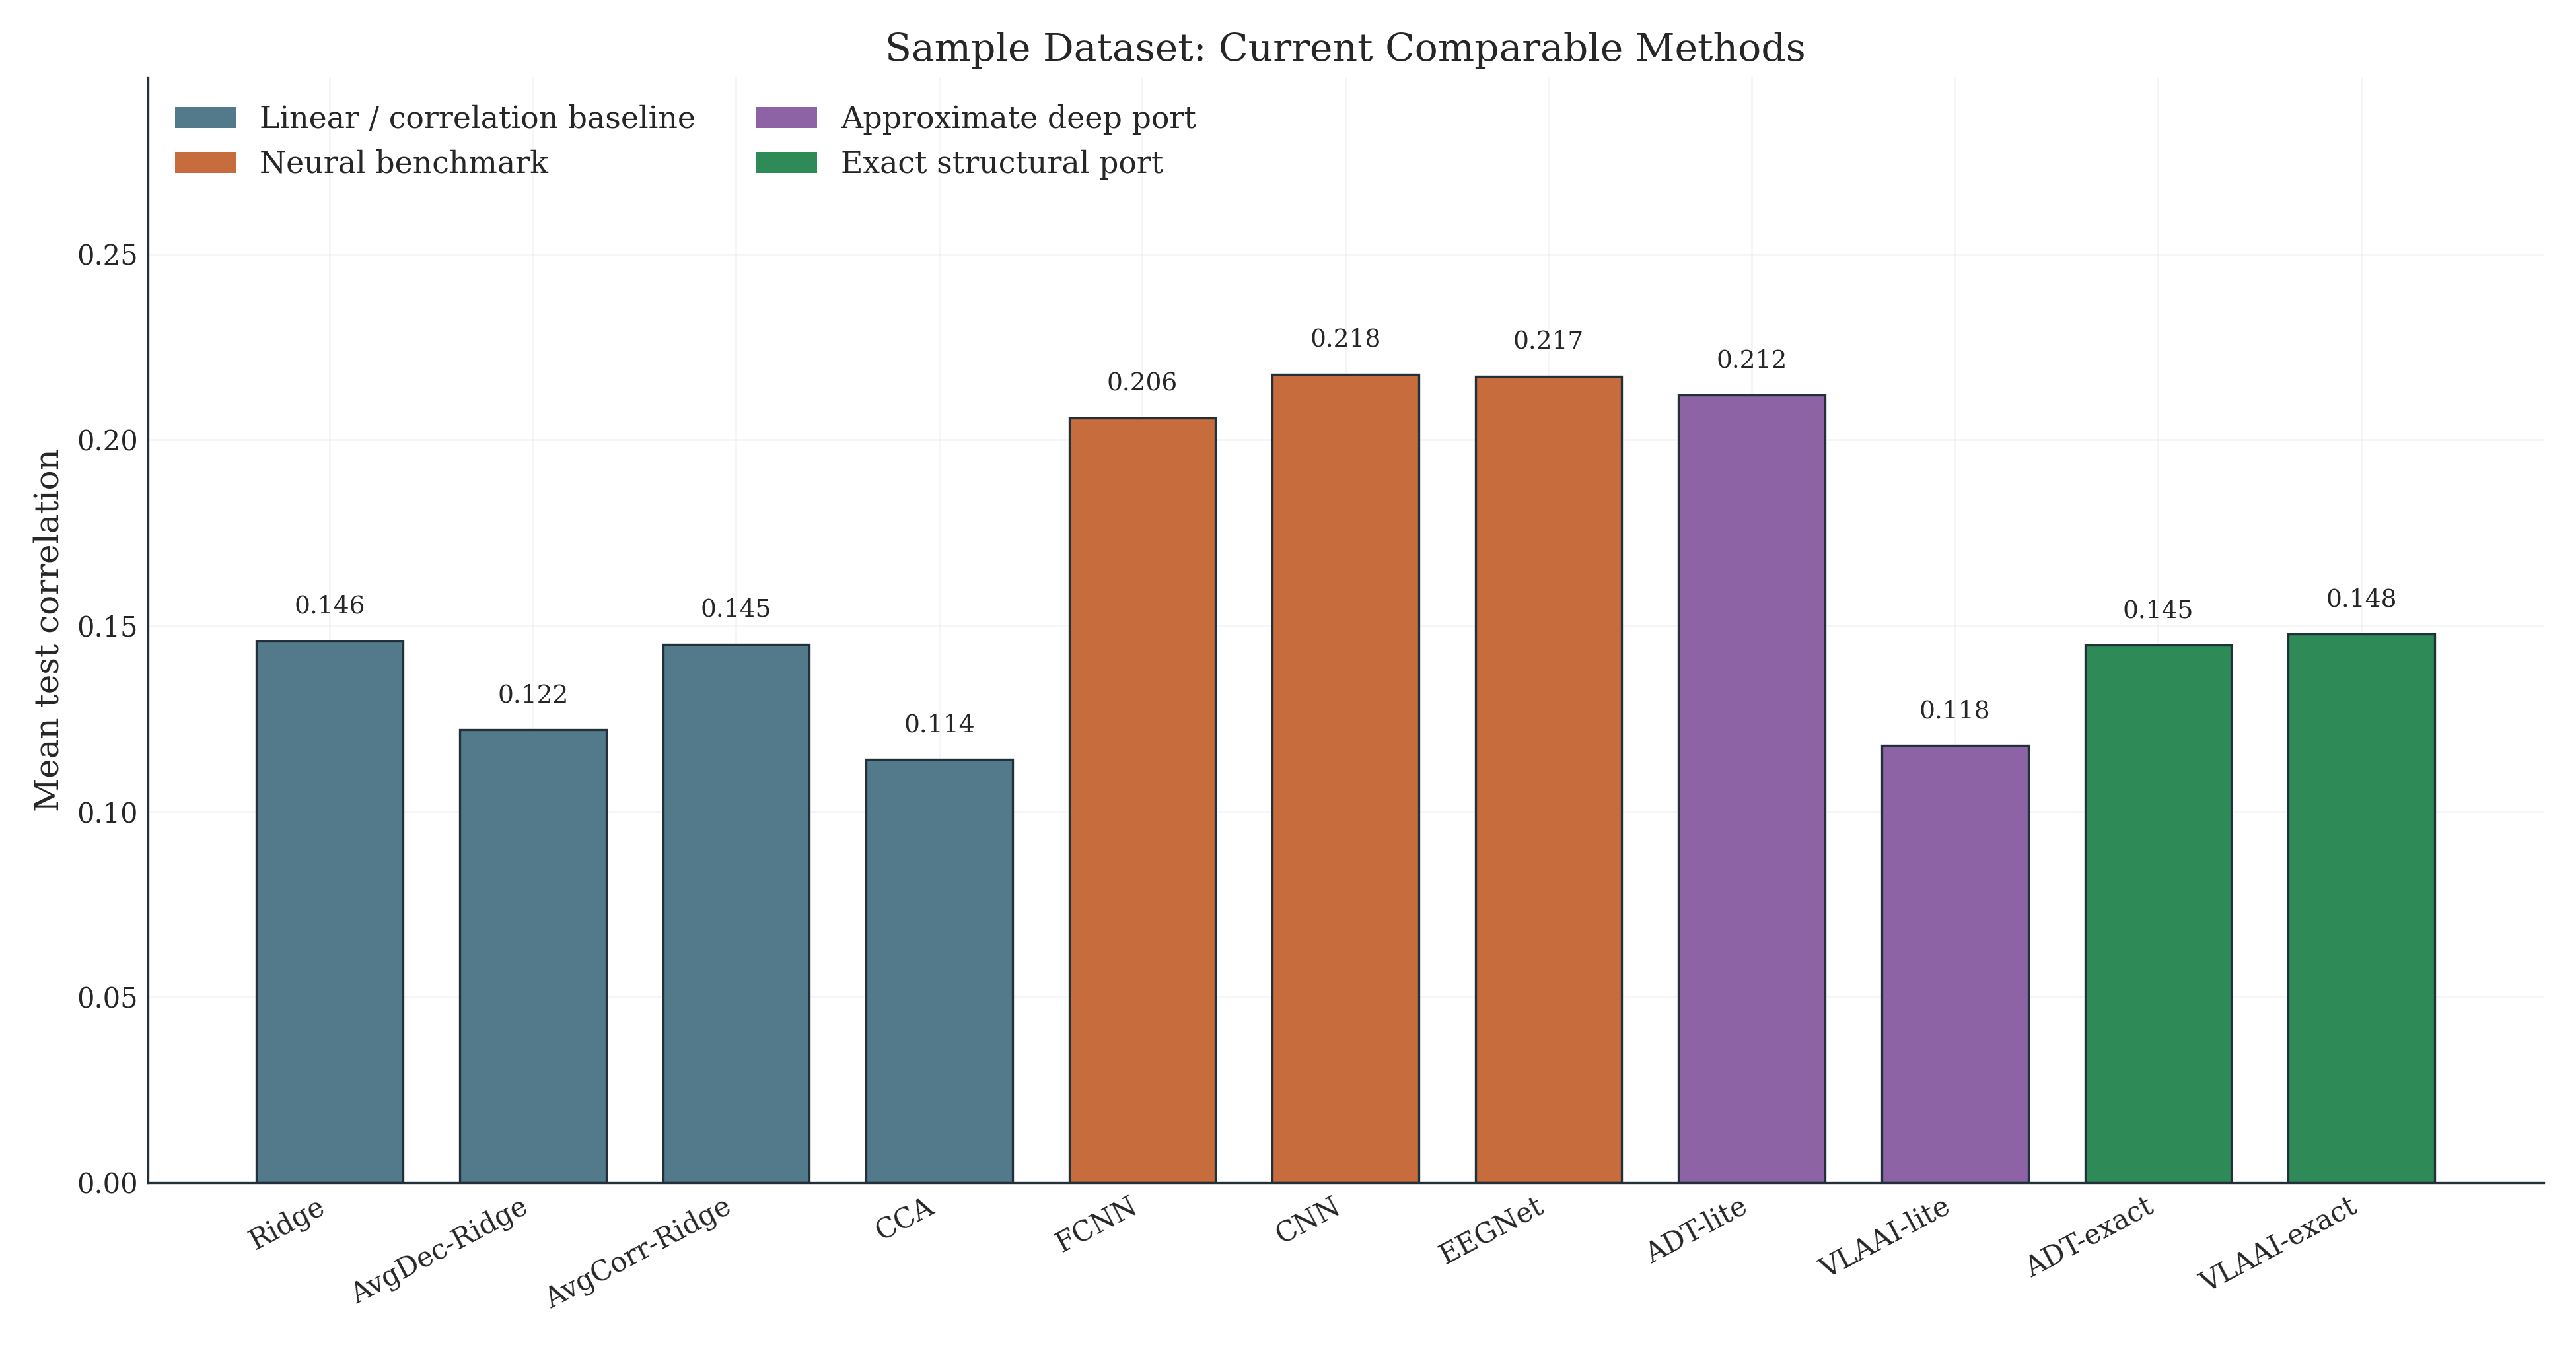
\includegraphics[width=\textwidth]{../experiments/summary_figures/sample_all_methods_overview.png}
\caption{Current comparable methods on the development sample dataset.}
\end{figure}

\section*{Exact-Port Cross-Dataset Table}
The exact structural ports can already be compared across the currently unified datasets:

\begin{longtable}{p{2.2cm} p{2.0cm} p{2.3cm} p{1.2cm} p{1.2cm} p{0.9cm}}
\toprule
Dataset & Model & Metric & Mean & Std & N \\
\midrule
\endfirsthead
\toprule
Dataset & Model & Metric & Mean & Std & N \\
\midrule
\endhead
hugo\_sample\_tf64 & ADT-exact & pearson\_metric & 0.1447 & 0.0416 & 13 \\
hugo\_sample\_tf64 & VLAAI-exact & pearson\_metric & 0.1477 & 0.0411 & 13 \\
weissbart\_tf64 & ADT-exact & pearson\_metric & 0.1147 & 0.0393 & 13 \\
weissbart\_tf64 & VLAAI-exact & pearson\_metric & 0.1389 & 0.0335 & 13 \\
etard\_tf64 & ADT-exact & pearson\_metric & 0.0860 & 0.0445 & 20 \\
etard\_tf64 & VLAAI-exact & pearson\_metric & 0.1128 & 0.0416 & 20 \\
\bottomrule
\end{longtable}

\section*{Interpretation}
At the current stage, the results support the following:
\begin{itemize}
\item the code paths run end-to-end on the unified datasets
\item \texttt{VLAAI-exact} is currently stronger than \texttt{ADT-exact} on both Weissbart and Etard
\item \texttt{EEGNet} is a strong baseline on the current reconstruction setup
\item \texttt{Ridge} remains competitive and should not be treated as a trivial baseline
\end{itemize}

\paragraph{What should not be over-claimed.}
The current results are meaningful, but they are not yet a final journal table because:
\begin{itemize}
\item pooled exact-port training and subject-specific baseline training are not identical regimes
\item scalar-window regressors and sequence-to-sequence models do not optimize exactly the same training target
\item the historical sample panorama includes shorter-budget development runs
\end{itemize}

\paragraph{Why different implementations can diverge substantially.}
This benchmark is sensitive to details that are easy to overlook:
\begin{itemize}
\item whether the prediction target is a single center/last-sample scalar or a full output sequence
\item whether training is subject-specific or pooled across participants
\item whether validation selects alpha, checkpoint epoch, or both
\item whether the metric is reconstruction correlation, canonical correlation, or match/mismatch accuracy
\item whether window length and hop length match the original implementation
\end{itemize}
Therefore, disagreement between two implementations is not automatically evidence of a bug. It may reflect a real protocol mismatch. This is exactly why the present package exposes both code pointers and run-level metadata.

At the same time, the current benchmark is not yet a final paper-ready leaderboard because:
\begin{itemize}
\item external generalization datasets are not yet integrated into the same adapter layer
\item true competing-speaker AAD datasets are not yet in the same reporting table
\item some sample-dataset baselines were historical short-budget runs and should be interpreted as development comparisons rather than final claims
\end{itemize}

\section*{Recommended Review Order}
A technically informed reviewer should inspect the package in the following order:
\begin{enumerate}
\item \texttt{docs/CURRENT\_EVALUATION\_STATUS.md}
\item \texttt{unified\_reference\_main\_summary.csv} and the corresponding figure
\item \texttt{reproduction\_audit\_training\_curves.csv} and the corresponding figure
\item \texttt{reproduction\_audit\_model\_protocols.csv}
\item \texttt{reproduction\_audit\_run\_metadata.csv}
\item the implementation files for the exact ports and the unified baseline runner
\end{enumerate}

\paragraph{Likely reviewer questions.}
The most important questions are likely to be:
\begin{itemize}
\item whether the exact ports are architecturally faithful enough
\item whether the pooled exact-port training regime is acceptable for the claimed comparison scope
\item whether the subject-specific baselines are being judged under a harder or easier setup than the exact ports
\item whether the observed validation curves look plausible rather than degenerate
\end{itemize}

\section*{Files Provided For External Review}
\begin{itemize}
\item \texttt{docs/CURRENT\_EVALUATION\_STATUS.md}
\item \texttt{experiments/summary\_figures/reproduction\_audit\_model\_protocols.csv}
\item \texttt{experiments/summary\_figures/reproduction\_audit\_run\_metadata.csv}
\item \texttt{experiments/summary\_figures/unified\_reference\_main\_summary.csv}
\item \texttt{experiments/summary\_figures/unified\_reference\_main\_overview.png}
\item \texttt{experiments/summary\_figures/reproduction\_audit\_training\_curves.csv}
\item \texttt{experiments/summary\_figures/reproduction\_audit\_training\_curves.png}
\item \texttt{experiments/summary\_figures/sample\_all\_methods\_summary.csv}
\item \texttt{experiments/summary\_figures/sample\_all\_methods\_overview.png}
\end{itemize}

\end{document}
